%\chapquote{"Video killed the radio star."}{The Buggles}{1979}

\section{Introduction}

\section{The Far-Infrared/Radio Correlation}

For samples of star forming galaxies in the local and high redshift universe there is a well observed correlation between the far-infrared and radio emission (e.g. \citealt{Dickey_1984}; \citealt{deJong_1985}; \citealt{Helou_1985}; \citealt{Condon_1992}; \citealt{Barger_2000}; \citealt{Yun_2001}; \citealt{Garrett_2002}; \citealt{Appleton_2004}; \citealt{Ibar_2008}; \citealt{Seymour_2009}; \citealt{Sargent_2010}), that remains nearly linear over multiple orders of magnitude in far-infrared luminosity ($10^{9} \lesssim L_{\textrm{FIR}} [L_{\odot}] \lesssim 10^{12.5}$). The small scatter in this relation is often attributed to the "calorimeter model" (\citealt{Voelk_1989}; \citealt{Lisenfeld_1996}; \citealt{Lacki_2010}), which ascribes the far-infrared and radio emission to common stellar sources. In this model, galaxies are assumed to be opaque to UV light from massive OB stars which gets absorbed by the dust in the ISM and reradiated in the far-infrared. Observations in the far-infrared and sub-mm are thus sensitive to the cold dust that reradiates the energy from young stars. These stars quickly come to the end of their lives, exploding as Type II supernovae producing cosmic ray electrons and positrons. Most of their energy gets radiated in the radio as synchrotron radiation when interacting with the magnetic fields of the supernova remnant. The radio continuum is therefore a tracer of recent, obscured star formation.

The appearance of a correlation at all redshifts and luminosities has facilitated studies that use the radio emission as an unbiased tracer of obscured star formation in dusty galaxies (\citealt{Kennicutt_2012}). By making use of the tight correlation (as well as the benefits we outline in the following section), we can identify counterparts to single dish sub-mm observations with large beams with greater confidence than we would expect from the optical or near-infrared. This allows for better characterization of the properties of SMGs and allows us to study the cosmic star formation history to higher redshifts (\citealt{Madau_2014}; \citealt{Delhaize_2017}; \citealt{Novak_2017}).

\section{Identifying Multiwavelength Counterparts to SMGs via Radio IDs}

As illustrated in Chapter \ref{chapter:Data_Release_3}, SMGs that are detected with single dish sub-mm telescopes with low angular resolution will likely include multiple galaxies in the optical or near-infrared within the beam width. This is a particular problem for \textit{Herschel} where even the smallest beam size at 250\,\micron\ has a FWHM of $\sim$ 18\,arcsec. The possibility of tightly clustered SMGs (\citealt{Blain_2004}) and with a higher surface density of optical counterparts, deciding unambiguously on the source of the sub-mm emission is difficult. This is further compounded by their intrinsic faintness due to the dust obscuration. The optimal way to overcome the problem of poor resolution is to follow up with millimetric or longer wavelength interferometric observations. In the following sections we detail a method for identifying radio counterparts to \textit{Herschel} sources in order to secure unambiguous multiwavelength counterparts to our sub-mm galaxies. The following is a list of benefits of using the radio emission to select counterparts throughout the electromagnetic spectrum.

\begin{enumerate}
    \item Star forming galaxies produce a lot of synchrotron emission. This allows us to take advantage of the FIRC to locate the galaxy emitting radiation in the far-IR. Compared to searches in other wavelengths, such as using the Likelihood Ratio to identify optical counterparts, the search for identifications is not solely motivated by their position and brightness, but also by the physical link between the two objects due to their common source.
    \item Even when considering the deepest radio maps, the low surface density of radio sources means that the probability of chance positoinal coincidences with a sub-mm source is relatively unlikely. As a result, we can have a reasonable confidence in some association between objects when we do observe radio sources in close proximity to the sub-mm position (\citealt{Ivison_2002}; \citealt{Borys_2004}). In most cases (as we shall validate in this study), radio sources are sufficiently rare that finding an object within the positional uncertainty of the sub-mm beam almost always results in a robust identification.
    \item When a secure radio counterpart is identified, the positional accuracy ($\sim$ 1\,arcsec for the Karl G. Jansky Very Large Array (VLA) at 1.4\,GHz and $\sim$ 0.75\,arcsec at 3\,GHz) allows for a unambiguous identification with an optical or infrared galaxy counterpart. By locating these galaxies via the radio identification, we predict a low false identification rate of the SMG with the optical counterpart, allowing us to determine their morphologies, colours, magnitudes, stellar masses and more with greater confidence.
\end{enumerate}

While the radio emission from star-forming galaxies allows for secure identification of counterparts across the spectrum, it also has several drawbacks. The following is a list of disadvantages to using radio emission.

\begin{enumerate}
    \item Our understanding of the radio-selected SMG population is likely to be skewed by selection effects. The negative k-correction in the far-infrared arises due to the steep Rayleigh-Jeans part of the SED and allows for nearly equal detection of dusty galaxies at $z \sim 0.5$ as $z \sim 8$ for longer wavelengths where this effect is most pronounced (\citealt{Blain_2002}). The radio, however, suffers from a strong positive k-correction which causes a bias against high redshift galaxies ($z > 3$). This means that a substantial fraction of SMGs remain undetected in the radio due to the lack of sufficiently deep radio data. Despite this, we note that such deep radio data would produce a redshift distribution of SMGs much wider than we could obtain with the coverage of the SGP in the near-infrared (Chapter \ref{chapter:Data_Release_3}).
    \item Despite the benefit of the FIRC in locating radio galaxies in close proximity to SMGs, the correlation also causes a preference for the brightest SMGs, which may not be a representative sample of the full SMG population.
    \item Interferometry has been used to show that for sub-mm sources in which we observe multiple radio galaxies in close proximity, in $\sim$ 80\% of cases the sub-mm emission is associated from only one of the radio sources. This leads to an ambiguity as to the nature of some apparent multiple systems when interferometry is not available.
    \item Potentially the most pivotal drawback for the identification of sub-mm emitting galaxies, is the sky coverage from radio surveys. While we have large sky surveys in the sub-mm such as \textit{Herschel}-ATLAS, using radio data for large area sub-mm surveys is not yet practical. Future radio surveys such as the Square Kilometre Array (SKA) and recent wide-area surveys with the Low-Frequency Array (LOFAR) allow us to produce larger samples of SMGs to understand their stellar properties.
\end{enumerate}

Many studies (e.g. \citealt{Eales_2009}; \citealt{Dye_2009}) adopt a frequentist approach to searching for possible radio counterparts close to the sub-mm position. This often involves using Monte Carlo simulations to estimate the probability that a given counterpart is located near the source by chance. The advantage of using a frequentist approach over a Bayesian method (Chapter \ref{chapter:Data_Release_3}) is that it does not require assumptions to be made on the form of the sub-mm positional errors, given that they are poorly known due to source confusion. As will be shown later, we can use the results of a frequentist approach to infer the distribution of positional errors. Despite this benefit, a frequentist approach would not have been appropriate for the VIKING counterparts we identified in the SGP because of their higher surface density.

\section{Identifying Radio IDs to \textit{Herschel} Sources in COSMOS}

In the following sections we identify radio counterparts to \textit{Herschel} detected sources in the Cosmic Evolution Survey (COSMOS). We applied the frequentist method of \citealt{Lilly_1999}, which differs from the Bayesian Likelihood Ratio method in that it searches for objects close to the sub-mm source and estimates the probability that each object is a chance alignment, rather than estimating the probability the two are physically associated. COSMOS is a deep, wide area survey of an equatorial two square degree field centered at R.A $+150.12^{\circ}$ and declination $+2.21^{\circ}$ (\citealt{Scoville_2007}). The field has been observed with many space-based (e.g. \textit{Hubble Space Telescope}, \textit{Spitzer}, \textit{Chandra} and \textit{Herschel}) and ground-based telescopes (e.g. Keck, VLA and UKIRT), resulting in multiwavelength data that spans from the X-ray to radio wavelengths. The high sensitivity and resolution of these data sets over a sufficiently large area, allows for comprehensive studies on the co-evolution of galaxies (\citealt{Schreiber_2018}; \citealt{Stockmann_2020}; \citealt{Valentino_2020a}), star formation (\citealt{Gruppioni_2013}; \citealt{Novak_2017}), large scale structure (\citealt{Scoville_2013}; \citealt{Laigle_2018}) and AGN (\citealt{Prescott_2006}; \citealt{Heintz_2016}). 

\subsection{\textit{Herschel} Observations in COMSOS}

The \textit{Herschel} detected sources that we study in this work were taken as part of the \textit{Herschel} Multi-tiered Extragalactic Survey (HerMES; \citealt{Oliver_2012}) {\color{red}Repeated from the introduction}. HerMES is a deep far-infrared imaging survey of some of the most well-studied blank extragalactic fields. As part of the survey, the COSMOS field was observed with SPIRE over the full two square degrees.

The survey design of HerMES allowed for the detection of a wide range in far-IR luminosities by targeting high luminosity objects which are bright but rare in wide, shallow surveys and the lower luminosity objects, which are faint but common, in deep, narrow surveys.

{\color{red}More description on the Herschel observations in the COSMOS field (HerMES) and the number of Herschel sources.}

\subsection{VLA Observations in COSMOS}

The VLA-COSMOS 3\,GHz Large Project (\citealt{Smolcic_2017a}; \citealt{Smolcic_2017b}; \citealt{Smolcic_2017c}) was a radio continuum survey covering 2.6 square degrees, enclosing the two square degrees of the COSMOS field, with a mean rms sensitivity of $\sim$ 2.4\,$\mu$Jy beam$^{-1}$ and an exceptional angular resolution of 0.75\,arcsec at 3\,GHz. Observations of the COSMOS field were taken in the S-band (2 -- 4\,GHz) for a total of 384 hours. The benefit of the S-band observations are the large effective bandwidth ($\sim$ 2\,GHz) and large field of view, allowing for fast coverage of a field such as COSMOS. The survey recovered 10,899 radio source components with SNR greater than five, 67 of which had been merged into multicomponent sources, resulting in a total of 10,830 radio sources. The VLA-COSMOS 3\,GHz catalgue builds on the existing 1.4\,GHz VLA catalogue (VLA-COSMOS Large and VLA-COSMOS Deep projects: \citealt{Schinnerer_2004}; \citealt{Schinnerer_2007}; \citealt{Schinnerer_2010}) of 2,865 1.4\,GHz-detected (L-band) radio sources. The increased sensitivity of the S-band compared to the L-band allows for an increase in the number of detected sources a factor approximately four times greater over a similar sky area, though we note that the sources detected in the VLA-COSMOS 3\,GHz catalogue are typically fainter.

The VLA-COSMOS 3\,GHz Large Project is the deepest radio continuum survey for a field as large as that of COSMOS, which combined with the extensive multiwavlength described above, makes it a unique survey for studying the composition of the radio-detected galaxy population. As we shall explore later, the \textit{Herschel}-detected sources that are coincident with radio sources in COSMOS make for an unparalleled set of far-IR selected galaxies with known stellar properties. With such confidence in the stellar properties of dusty star forming galaxies, this data set provides an opportunity to precisely determine the galactic environments conducive to such high star formation rates and allow us to make predictions about the radio populations from future surveys that will be able to cover the larger areas of sky already mapped in the far-IR and sub-mm. The robust radio IDs to \textit{Herschel} sources will help facilitate the identification of similar dusty galaxies in large surveys from the likes of the SKA (\citealt{Dewdney_2009}) and the Next Generation Very Large Array (ngVLA), as well as their precursors such as the Australian Square Kilometre Array Pathfinder (ASKAP: \citealt{Johnston_2007}), the \textit{enhanced} Multi Element Remotely Linked Interferometer Network (\textit{e}-MERLIN), LOFAR and MeerKAT (\citealt{Jonas_2009}).

The sample studied here are the \textit{Herschel}-detected and VLA-detected sources that lie within an overlapping region as shown in Figure \ref{fig:sky_map}. We define a square region from R.A $+149.29^{\circ}$ to $+150.95^{\circ}$ and declination $+1.45^{\circ}$ to $+3.04^{\circ}$. This 2.64 square degree region contains 7,230 (64.6\%) \textit{Herschel} and 10,826 ($\sim$ 100\%) radio sources.

\begin{figure}
	\centering
	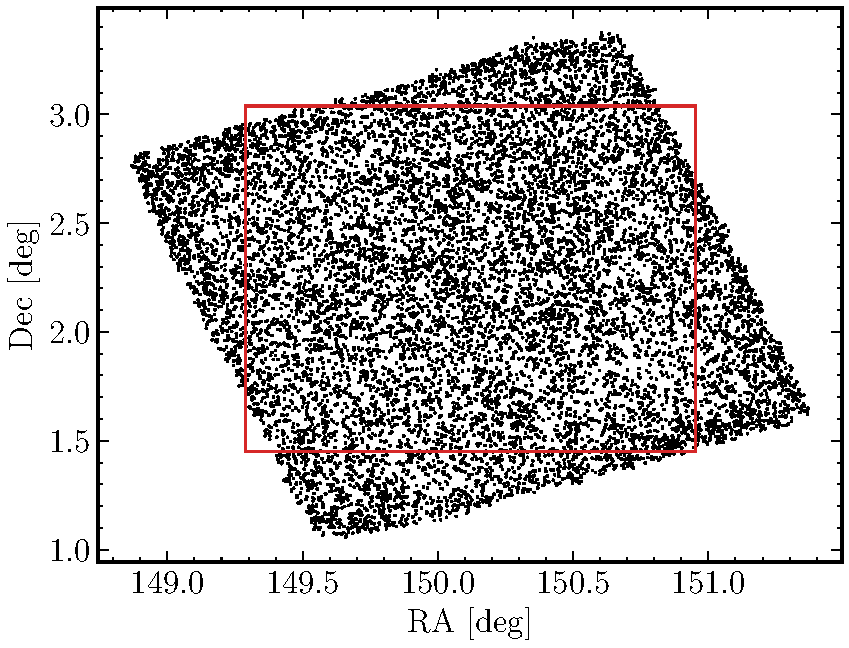
\includegraphics[width=0.75\columnwidth]{Figures/sky_map.pdf}
	\caption{The map of \textit{Herschel} detections (black points) and the area covered by the VLA observations (red square). There are a total of $11,185$ \textit{Herschel} sources, of which $7,230$ ($64.6$\%) lie within the region covered by the VLA-COSMOS $3\,$GHz Large Project.}
	\label{fig:sky_map}
\end{figure}

\subsection{The COSMOS2020 Catalogue}

{\color{red}A brief description of the COSMOS2020 catalogue. Include: i) Available photometric bands ii) SED fitting (for stellar masses)}

\subsection{Calculating the Significance of Associations}
\label{sec:radio_significance}

To predict the probability that a sub-mm-radio pair is a significant association we could use the corrected Poisson probability defined by \citealt{Downes_1986}. This measures the Poisson probability that a radio source of a given flux density could lie at the observed distance from the source by chance. In this original paper the Poisson probability is defined as $P = 1-e^{-\mu}$ where $\mu = \pi r^2n$. Here $r$ is the radial offset between the source and radio counterpart and $n$ is the surface density of objects brighter than the radio counterpart. While a low value of $P$ does not confirm that the radio source is the correct ID for the sub-mm source, it suggests that the two are likely associated. A low value of $P$ can be interpreted in a number of ways. First, the radio source could be the true counterpart of the sub-mm source. Second, the counterpart could be one of a group of galaxies that collectively contribute to the flux density observed in the sub-mm. This is a very plausible case for the sources in our sample given the large beam sizes for \textit{Herschel}-SPIRE. Third, the low value of $P$ could be the result of an indirect association with the source, for example, due to clustering with the true ID or from the effects of gravitational lensing (although in the case of gravitational lensing this seems unlikely for our sample, as this would suggest that the lenses are as dust obscured as the background sources).

We used the method of \citealt{Lilly_1999} which applies the principles of the Poisson probability from \citealt{Downes_1986} in a Monte Carlo approach. The method, which is given in detail in \citealt{Dye_2009}, is as follows. First, we generate a set of $N$ random positions in the area common to both the sub-mm and radio surveys. Next, we identify all radio sources within some maximum radius, $r_{\textrm{max}}$, from each random position. For each radio source we measure the quantity $S = r^2n$, where $r$ and $n$ take the same definitions as earlier. The minimum value of $S$ for each source (corresponding to the most significant association in the case where multiple radio sources are observed) is retained. This defines our distribution, $D(S)$, which represents the distribution of $S$ values for random chance alignments. This distribution allows us to determine the probability of an observed radio source with $S = S_i$ and within $r_{\textrm{max}}$ of a sub-mm source being a random interloper. This is computed as:

\begin{equation}
    P(< S_i) = \frac{1}{N}\int_0^{S_i}D(S) dS.
    \label{eq:probability_frequentist}
\end{equation}

As is often assumed, we consider a radio source to be a secure identification if it has $P < 0.05$, suggesting that there is less than a 5\% probability that such a radio source would be observed by chance (e.g. \citealt{Ivison_2002}; \citealt{Ivison_2005}; \citealt{Pope_2006}). Depending on the surface density of radio galaxies, the maximum value of $P$ will often be less than one as some fraction of the randomly chosen positions will not contain any radio sources within $r_{\textrm{max}}$. 

The value of $r_{\textrm{max}}$ is an important choice. While a smaller search radius reduces the number of potential IDs and increases the likelihood of missing a true counterpart, a larger radius causes a greater probability of observing a background object and thus matching the source with an unrelated radio galaxy. A further problem is that too large a search radius causes overlapping fields which could lead to radio sources being connected to more than one sub-mm position. Previous studies (e.g. \citealt{Dye_2009}) have defined the maximum radius using a probabilistic balance between these two competing effects, finding the radius where the expected number of false counterparts in the final sample equals the expected number of true counterparts that are excluded. In this study we are attempting to define a clean sample of radio matched \textit{Herschel} sources, such that our multiwavelength counterparts from the COSMOS field represent a near complete and thorough description of the optical to radio properties of \textit{Herschel} detected sources. As we shall show later, this sample could provide a useful starting point for identifying dusty galaxies in future large area surveys (e.g. \textit{Euclid}) given that our sample will define some subpopulation of the COSMOS survey. For this reason, we are less interested in retaining the appropriate size of the sample, but rather in minimizing the number of falsely identified counterparts that would obfuscate our picture of dusty galaxies. 

Figure \ref{fig:optimal_radius} shows the radial distribution of VLA sources from the 7,230 \textit{Herschel} positions. Also shown is the number of matches with 7,230 random positions. The peak at small separations illustrates the excess of true counterparts over the background level. At larger separations the number of matches with \textit{Herschel} positions follows the linear relation observed around random positions. The number of VLA sources observed at $r \sim 10$\,arcsec from \textit{Herschel} positions and random positions is approximately equal, corresponding to the radial offset beyond which we expect the probability of a counterpart being associated with the source is dominated by chance alignments. This radius may seem prone to misidentification, but if we consider the cumulative number of counterparts to a search radius $r$ (inset figure), then we see that a maximum search radius of $r_{\textrm{max}} \approx 10$\,arcsec corresponds to a maximum in the excess of expected true counterparts over background sources. This implies that at this radius the number of counterparts observed within the search radius is dominated by true counterparts, which will aid in reducing the false identification rate.

\begin{figure}
	\centering
	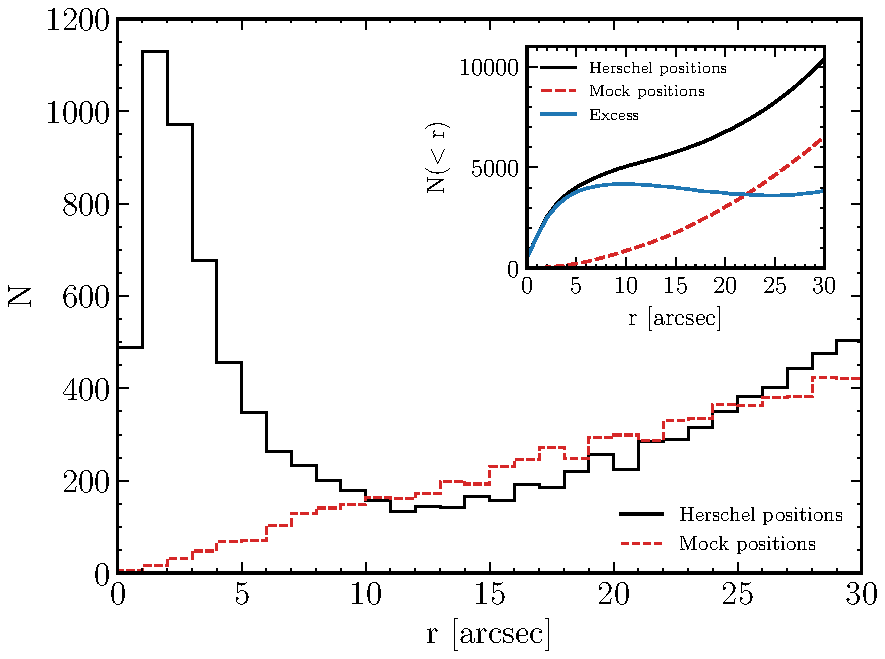
\includegraphics[width=0.75\columnwidth]{Figures/optimal_radius.pdf}
	\caption{The distribution of radial offsets between \textit{Herschel} sources and radio sources (black hatched histogram) and between VLA sources and random positions in the COSMOS map (red dashed line). The inset panel shows the cumulative distributions for the two histograms and the difference between them (blue solid line). The excess number of radio sources above the background decreases beyond $\sim10\,$arcsec. Therefore, we choose $r = 10\,$arcsec as our maximum search radius.}
	\label{fig:optimal_radius}
\end{figure}

Given that our VLA observations have a surface density of $4103\,$deg$^{-2}$ and we are assuming a maximum search radius of 10\,arcsec, we can approximate the maximum value of $P$. As a first order approximation, the maximum $P$ value is equal to the ratio between the probability of observing at least one VLA source within the search radius of a random position and the probability that the position is a blank field. Assuming Poisson statistics with a mean number of counterparts per random position of $\lambda = N_{\textrm{VLA}}A_{\textrm{random}}/A_{\textrm{survey}}$, where $N_{\textrm{VLA}}$ is the number of VLA sources, $A_{\textrm{random}}$ is the search area around a random position and $A_{\textrm{survey}}$ is the total survey area, then an estimate of $P_{\textrm{max}}$ can be given by:

\begin{equation}
    P_{\textrm{max}} \approx \frac{P(\textrm{Not Blank})}{P(\textrm{Blank})} = \frac{P(X > 0)}{P(X = 0)} = \frac{1 - P(X = 0)}{P(X = 0)} = \frac{1 - e^{-\lambda}}{e^{-\lambda}} \approx 0.10,
\end{equation}

\noindent where $X$ is the number of VLA sources observed around each random position. This calculation suggests that the maximum $P$ value for any radio source observed near a \textit{Herschel} source is $0.1$, not considering effects such as clustering, multicomponent galaxies or overlapping search areas. The fact that only $\sim$ 10\% of random positions will be incident with at least one radio source gives further confidence in the association between any \textit{Herschel} and VLA sources in close proximity.

\section{Results of the Frequentist Method Applied to \textit{Herschel} Sources}

We apply the method described above to all possible VLA counterparts within 10\,arcsec of a SPIRE source. We retain all counterparts that have $P < 0.05$, but consider as our primary counterparts those with the lowest $P$ value per \textit{Herschel} source. Figure \ref{fig:ds_distributions} shows the distribution of $S$ for radio counterparts to \textit{Herschel} (black histogram) and $10^6$ random positions (red histogram). The clear offset between the two distributions illustrates how a large fraction of the counterparts identified in the radio trace the sub-mm sources.

\begin{figure}
	\centering
	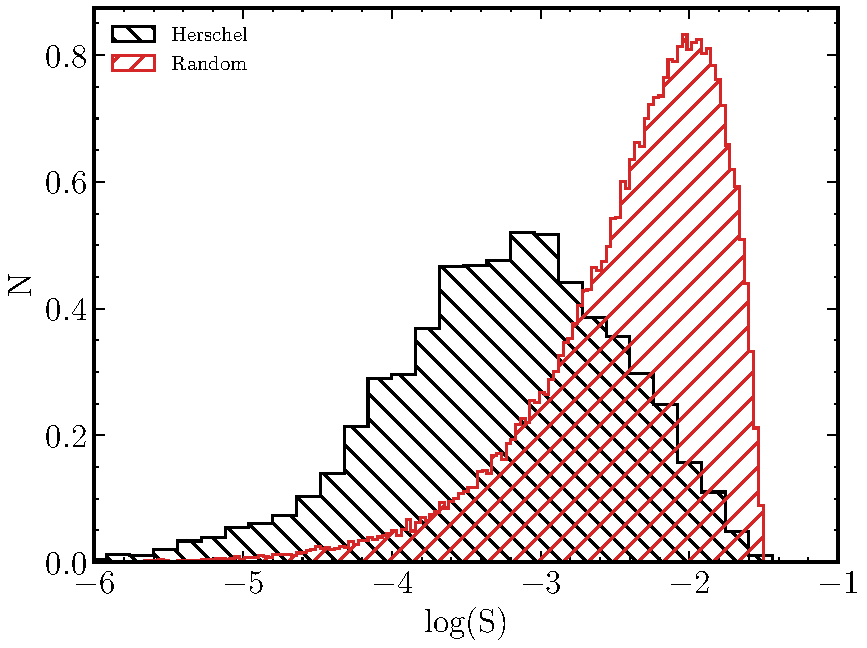
\includegraphics[width=0.75\columnwidth]{Figures/ds_distributions.pdf}
	\caption{The distribution of log(S) for the most likely counterpart lying within $10\,$arcsec of the position of a \textit{Herschel} source (black histogram) and a random position (red histogram). The offset between the two distributions highlights the fact that many radio counterparts with low S are truly associated with the \textit{Herschel} source.}
	\label{fig:ds_distributions}
\end{figure}

The total identification rate, that is the number of sources identified with $P < 0.05$ by a radio source, is 3,787/7,230 (52\%). However, the identification rate is a strong function of the sub-mm flux density (Figure \ref{fig:id_rate}). There is a strong decline toward fainter 250\,\micron\ fluxes ($< 30\,$mJy) where we approach the confusion limit of the survey. To be consistent with our motivation for a clean and unambiguous sample of \textit{Herschel} galaxies and their multiwavelength properties, we henceforth refer only to the sources with 250\,\micron\ flux densities greater than 30\,mJy, where we are more confident that they correspond to true sources. The survey area corresponds to 1,324 \textit{Herschel} sources with $S_{250\,\mu m} > 30\,$mJy. Of these sources, 1,053 (80\%) have radio IDs with $P < 0.05$.

\begin{figure}
	\centering
	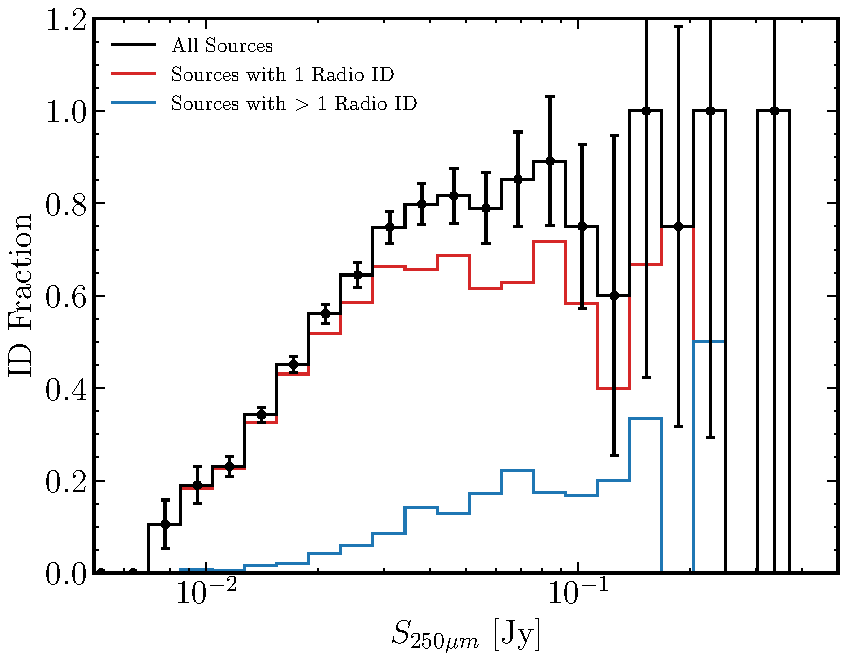
\includegraphics[width=0.75\columnwidth]{Figures/id_fraction_radio.pdf}
	\caption{The identification rate of \textit{Herschel} sources with radio counterparts as a function of $250\,\mu$m flux density. The black line shows the identification rate for all \textit{Herschel} positions, while the red and blue lines represent the fraction of those sources that have one or multiple radio counterparts with $P < 0.05$, respectively.}
	\label{fig:id_rate}
\end{figure}

Given that $P_i$ represents the probability of observing a radio counterpart, $i$, with a given flux and offset from the source by chance, the number of false IDs in a $P$-limited sample is given by

\begin{equation}
    N_{\textrm{False}} = \sum_{P_i < 0.05} P_i,
    \label{eq:false_radio_ids}
\end{equation}

\noindent which is analogous to Equation \ref{eq:false_ids} when using the LR method. From this we estimate that the false identification rate is approximately 0.5\% ($N_\textrm{False} \approx 7$). Compared to the fraction of false reliable counterparts identified in the near-IR as part of the H-ATLAS SGP ($\sim$ 4.8\%), the cleanness of the radio sample appears to be much higher. One of the driving factors of this difference is the surface density of radio sources compared to near-IR galaxies. The average number of potential counterparts per source for the VIKING analysis was $\sim 5.2$ (1,005,359 counterparts to 193,527 sources), which if we scale to a search radius of 10\,arcsec reduces to $\sim 2.1$ assuming they are uniformly scattered across the survey. By comparison, there are approximately 1.5 radio sources for each \textit{Herschel} source in COSMOS (10,826 counterparts to 7,230 sources).

While the above estimate of the false ID rate was computed for those counterparts with the lowest value of $P$ per source (the "primary" sample), we also observe secondary and tertiary associations that also have $P < 0.05$. For the 1,053 sub-mm sources that have robust identifications, 879 (83.5\%) have just a single association, 160 (15.2\%) have two and 14 (1.3\%) have three. The straightforward interpretation of single counterparts is that the radio source is the sole location of the far-IR emission. This is further supported if the counterpart is especially bright and close to the source, this would suggest that we are not likely to be mistaken by confusion or by larger offsets that may suggest missing secondaries that are below our detection. However, the nature of the multiple systems is less obvious and is explored in Section \ref{sec:multiple_systems}.

{\color{red}Briefly talk about the crossmatching with COSMOS2020 so we can talk about i) redshift distribution, ii) stellar mass distribution}

\subsection{Positional Errors and the \textit{Herschel}-SPIRE Point Spread Function}

The excellent accuracy of the 3\,GHz VLA sources (angular resolution of 0.75\,arcsec) means that the distribution of the offsets between the source position and the counterparts can be assumed to be an approximation of the sub-mm positional errors. As demontrated in Chapter \ref{chapter:Data_Release_3}, the \textit{Herschel}-SPIRE point spread function (PSF) is often assumed to take the form of a Gaussian, which we have previously estimated to have a width of $\sigma \sim 2.4$\,arcsec at $250\,\mu$m. In the following we use our set of robust radio identifications to validate this claim.

Figure \ref{fig:source_counterpart_offset} shows the positional offsets for the radio data from the sub-mm location. The solid line shows the offsets for all primary counterparts, the dotted line for all associations including secondaries and tertiaries, and the dashed line shows the average offset of all radio counterparts for each \textit{Herschel} source. On the assumption of Gaussian errors in R.A. and Dec, and if the distribution of radial offsets truly originates from random uncertainties in the position of the sub-mm source, then the distribution of radial offsets should resemble a Rayleigh distribution of the form $R(r, \sigma) \propto \frac{r}{\sigma^2}e^{-\frac{r^2}{2\sigma^2}}$. This results from the fact that for two independent Gaussian random variables with mean zero and standard deviation $\sigma$, as we might expect for the offset in R.A. and Dec ($\Delta\alpha$, $\Delta\delta$), then the offset defined as $r = \sqrt{\Delta\alpha^2 + \Delta\delta^2}$ has a Rayleigh distribution with parameter $\sigma$. The distribution of positional offsets from the sub-mm position for the primary radio sources is well described by a Rayleigh distribution with a width $\sigma = 1.66\,$arcsec (red line). This is substantially lower than our estimate of the 1$\sigma$ positional error measured in Chapter \ref{chapter:Data_Release_3} ($\sigma_{\textrm{pos}} = 2.388\pm0.065$\,arcsec). The corresponding Rayleigh distribution with $\sigma = 2.388$ for the same number of counterparts is illustrated with the green line in Figure \ref{fig:source_counterpart_offset}. This represents the expected distribution of radio offsets assuming the form of the source positional errors, $f(r)$, that is typically used in previous \textit{Herschel}-ATLAS studies (we refer the reader to Figure \ref{fig:Q_estimate}). {\color{red}However, we are reminded that our estimate of $\sigma_{\textrm{pos}}$ from the LR method relied on counting the number of blank sub-mm positions observed on the near-IR images, which is much shallower than the radio data used here. The median redshift of our near-IR counterparts was $\sim 0.49$, while the median redshift of our radio detected sample is $\sim 0.91$. By scaling the value of $\sigma_{\textrm{pos}}$ by the physical distance this corresponds to at the median redshift of the radio IDs, we predict that the positional error should be $\sigma_{\textrm{pos}} \sim 1.85$. The rescaled Rayleigh distribution is illustrated as the dashed green line. We see that this expected distribution is in much better agreement with our measurement of the positional errors. This suggests that in the absence of any knowledge of the sub-mm positional error distribution, the LR method retrieves a reasonable function for $f(r)$ that mostly resembles the distribution we observe from astrometrically precise radio positions.}

{\color{red} Need something to replace the above.}

\begin{figure}
	\centering
	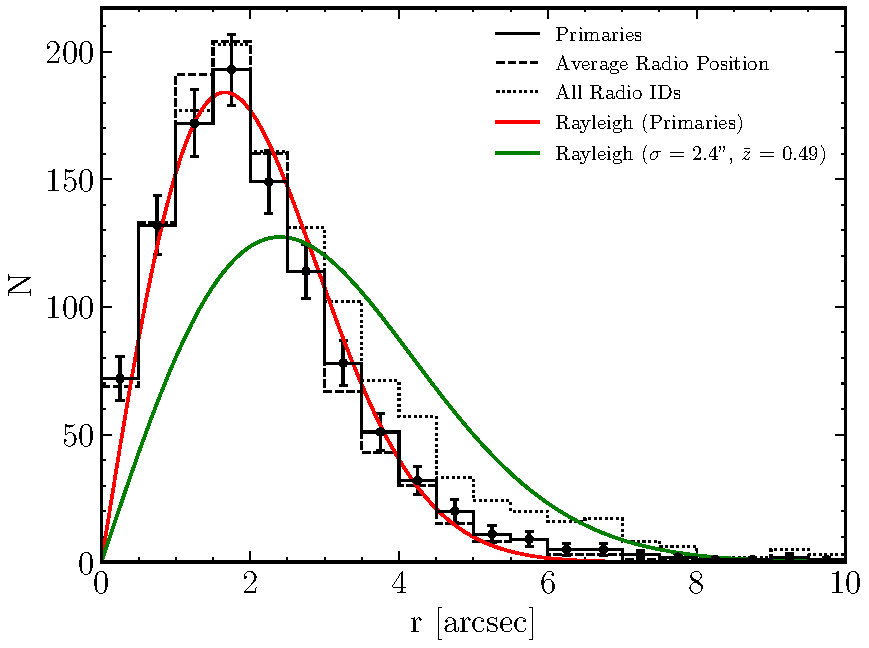
\includegraphics[width=0.75\columnwidth]{Figures/source_counterpart_offsets.pdf}
	\caption{The distribution of positional offsets from the \textit{Herschel} position for the radio sources with $P < 0.05$. The solid black histogram shows the distribution for the primary radio counterparts (those with the lowest $P$ value per \textit{Herschel} source), the dotted black histogram represents all radio IDs (including secondary and tertiary counterparts), and the dashed black histogram represents the radial offset between each \textit{Herschel} source and the average radio position. The latter provides a better description of the positional offsets for multicomponent sources. The red line shows a Rayleigh distribution, $R \propto r/\sigma^2 e^{-r^2/2\sigma^2}$, fitted to the primary counterparts. As detailed in the text, the value of $\sigma$ from the Rayleigh distribution ($\sigma = 1.66\,$arcsec) is a suitable estimate of the \textit{Herschel}-SPIRE $250\,\mu$m positional error. We compare this to a Rayleigh distribution with a standard deviation of the positional errors equal to $2.4\,$arcsec, as found in Chapter \ref{chapter:Data_Release_3}.}
	\label{fig:source_counterpart_offset}
\end{figure}

\subsection{The Nature of Multiple Identifications}
\label{sec:multiple_systems}

For roughly one sixth of sources, the correct identification is not obvious due to secondary and possibly tertiary candidates with a low probability of occurring by chance. There are several interpretations of such multiplicity. One possible explanation is that the radio sources are gravitationally lensed images of the far-IR emitting galaxy, but as mentioned earlier, this is unlikely. Other possibilities include clustering of true associations or unrelated counterparts that are flux boosted in the sub-mm by confusion noise. Determining unambiguously whether \textit{Herschel} sources with multiple identifications are predominantly physically associated or the result of confusion would require spectroscopic data. A number of studies have suggested that SMGs are strongly clustered (e.g. \citealt{Blain_2004}; \citealt{Weiss_2009}) while other studies suggest that multiple associations can be explained solely by the low angular resolution of single-dish observations (e.g. \citealt{Williams_2011}). Studies using interferometric observations at millimeter wavelengths have already shown that $\gtrsim$ 20\% of sub-mm sources correpsond to multiple SMGs that have been blended in single-dish observations (\citealt{Karim_2013}; \citealt{Simpson_2015}; \citealt{Stach_2018}). 

We attempt to understand the nature of our multiple systems by considering two questions: i) are all multiple counterparts to a source real? ii) are the counterparts, if physical, associated with each other? First, we note that the ID fraction of sources with multiple counterparts (Figure \ref{fig:id_rate}) is not restricted to low 250\,\micron\ flux densities, suggesting that most of the sources are real and thus their multiplicity is a product, either directly or indirectly, of a real sub-mm source. The ID fraction increases with flux density, which is not surprising since the inclusion of emission from multiple SMGs will only increase the total flux. The fractional contribution of the brightest radio ID to the total 3\,GHz flux density is plotted as a function of the 250\,\micron\ source flux density in the top panel of Figure \ref{fig:multiples_flux_contribution}. The median and standard deviation in the distribution of fractional contributions to the total 3\,GHz flux density is shown by the black error bars for the brightest radio component, and as red and blue lines for the second and third components, respectively. Some sources appear to have radio components where one counterpart dominates the radio flux ($\gtrsim 90\%$). In these cases we may presume that the sub-mm source corresponds to the bright radio object thanks to the well defined far-IR/radio correlation, and the minor components can effectively be ignored (or are chance background sources). However, the majority of our brightest counterparts contribute $\sim 50 - 70\%$ with significant contributions coming from secondary and possibly tertiary associations. The interpretation here is that the sub-mm emission emanates from more than one SMG that have been blended together by the \textit{Herschel}-SPIRE beam.

\begin{figure}
	\centering
	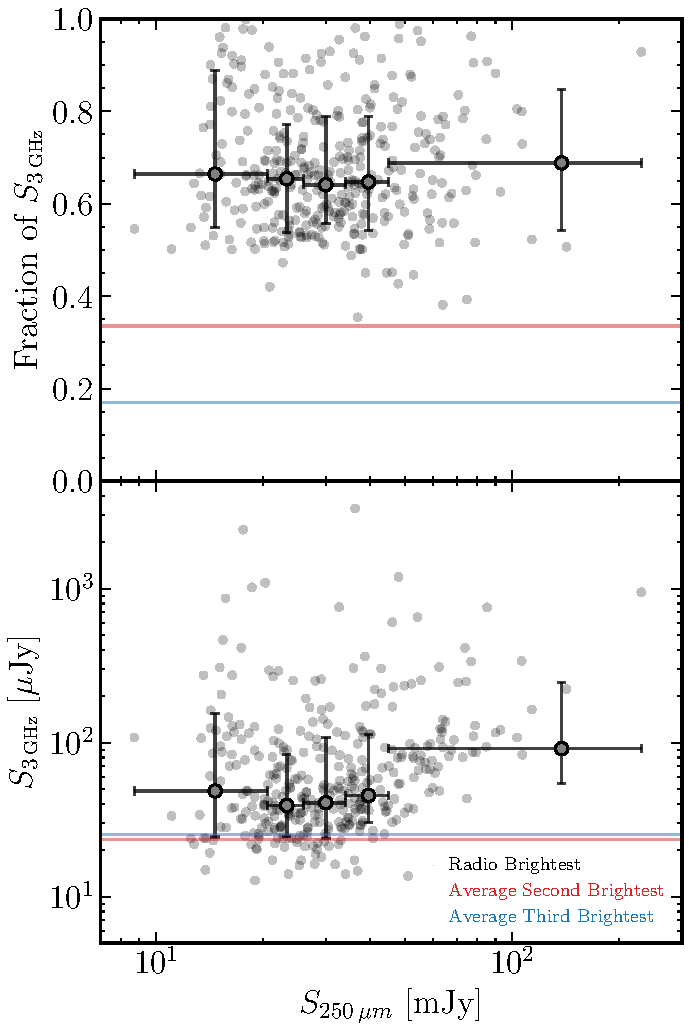
\includegraphics[width=0.75\columnwidth]{Figures/multiples_flux_contribution.pdf}
	\caption{The fraction of the integrated $3\,$GHz flux contributed by the brightest radio counterpart, as a function of the $250\,\mu$m flux of multicomponent \textit{Herschel} sources (top panel). The median contribution by the second and third brightest components are shown with red and blue lines, respectively, while the median contribution from the brightest radio sources is illustrated by a series of error bars. The vertical errors correspond to the 16th to 84th percentiles. The bottom panel illustrates the raw radio flux.}
	\label{fig:multiples_flux_contribution}
\end{figure}

There appears to be no dependence of the median flux fraction of the brightest component on the total 250\,\micron\ flux. Previous studies (e.g. \citealt{Scudder_2016}) have suggested that the fractional contribution increases toward low source flux density, but there is only weak evidence here. The bottom panel of Figure \ref{fig:multiples_flux_contribution} shows the raw flux of all the brightest components as a function of the total 250\,\micron\ flux density. It is not unexpected that the brightest \textit{Herschel} sources also have the brightest radio IDs, however, due to the near constant flux contribution, this suggests that in the brightest sub-mm sources we observe multiple bright objects that all have elevated radio fluxes. This might suggest the presence of a group or cluster of galaxies. Interestingly, at mid- to low-flux sources, the brightest component has a near constant radio flux density, though this is likely influenced by the differing observable depths of the \textit{Herschel} and VLA observations.

In Figure \ref{fig:multiples_separation} we plot the radial separation between the two IDs as a function of the difference in the photometric redshift of the counterparts, if contained in COSMOS2020. The high percentage of sources that have secure radio IDs with redshifts within 0.1 of each other suggests that a significant fraction of the sub-mm sources that resolve into multiple SMGs are indeed physically associated with each other. The scatter at larger redshift separations suggests a significant fraction of sources with random interlopers. There appears little preference for small or large angular separations, though the corresponding physical scale depends on the redshift of the source. For the median redshift of our counterparts, we observe multiple components that are at the same redshift being separated by physical distances between $\sim$ 10 and 100\,kpc. The prevailing theory for SMG formation is that they are the result of major mergers (\citealt{Ivison_2002}; \citealt{Smail_2004}; \citealt{Ivison_2007}; \citealt{Engel_2010}; \citealt{Hayward_2011}) that induce a starbursting phase and boost the sub-mm flux. The lack of very small offsets suggests that these components are not likely to be lensed images, but could be interacting galaxies and mergers, and given the large range of separations, may further indicate the presence of clusters of galaxies.

\begin{figure}
	\centering
	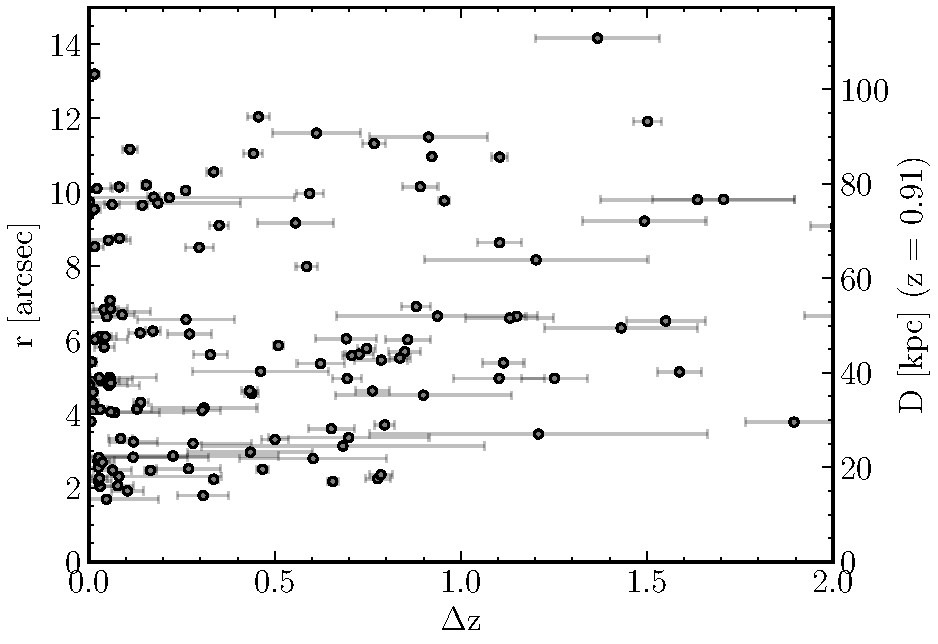
\includegraphics[width=0.75\columnwidth]{Figures/multiples_separation.pdf}
	\caption{\textit{Herschel} sources with multiple $P < 0.05$ radio counterparts in the plane of $\Delta z$ and $r$, representing the difference in the photometric redshift of the radio sources and the separation from each other. The top panel shows the histogram of $\Delta z$. This figure illustrates that those \textit{Herschel} sources with multiple associations have radio separations between $\sim 10$ and $100\,$kpc (at an average redshift of $z = 0.91$) and are predominantly detected at the same redshift.}
	\label{fig:multiples_separation}
\end{figure}

\subsection{Missing Identifications}

For 271 \textit{Herschel} sources ($> 30\,$mJy) we do not observe any radio counterpart within 10\,arcsec of the sub-mm position, or we observe a potential counterpart, but it is not considered a robust association ($P < 0.05$). This corresponds to approximately 20\% of the total sample. If we allow the counterparts to be considered secure to $P < 0.1$, then the number of blanks reduces by only 17 sources to 254. From our calculation in Section \ref{sec:radio_significance}, this corresponds to any object being observed within the search radius being considered robust, which tells us that the majority of our blank fields are not due to a large number of tentative crossmatches, but a result of a number of sub-mm positions where no possible radio counterparts are observable.

There are several reasons why we might not observe true counterparts. The most obvious reason is that a small number of sub-mm detections are likely to be spurious, though we remove most of this problem by considering sources with $S_{250} > 30\,$mJy. Secondly, the true counterpart could lie outside of the search radius. {\color{red}Quick calculation on the number of true IDs we predict beyond 10 arcsec?} Another possibility is that the SMG lies at $z > 3$, beyond the depth of our 3\,GHz observations (\citealt{Eales_2003}). We can test this possibility by comparing the radio-detected and radio-undetected sub-mm source populations. Figure \ref{fig:blank_fir_colours} shows a \textit{Herschel} colour-colour plot for the sources in which we observe at least one radio ID and those in which the field is blank to $P < 0.05$ counterparts. For illustration purposes, we show the path taken by a galaxy with a dust temperature of 30\,K and dust emissivity index, $\beta = 2$, from $z = 0$ to $z = 4$ (right to left). There is no clear difference between the two populations, suggesting that the blanks are not necessarily at higher redshifts. We note, however, that the same colour-colour diagram would be observed if the blank sources represented SMGs with typically colder characteristic dust temperatures (\citealt{Chapman_2004}) at lower average redshifts.

\begin{figure}
	\centering
	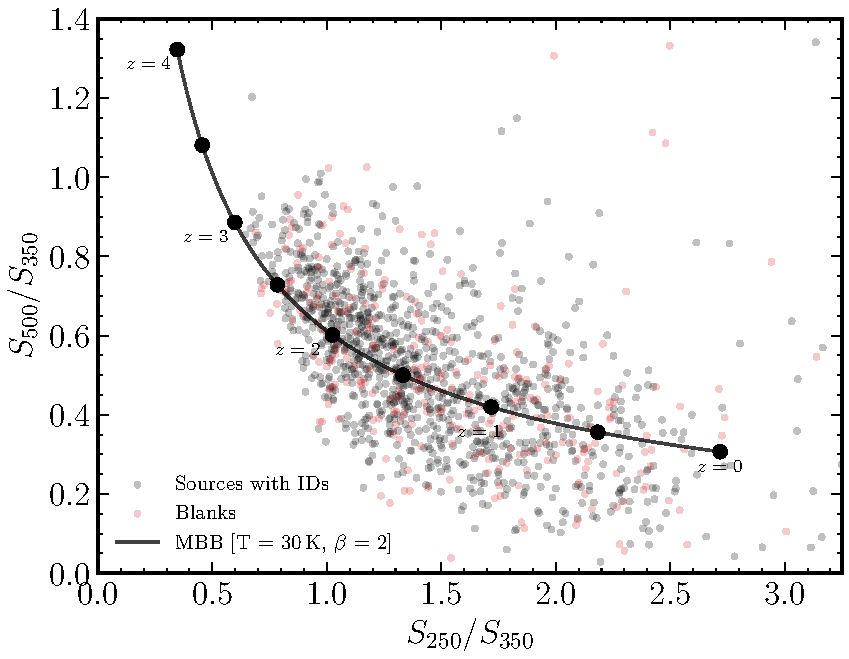
\includegraphics[width=0.75\columnwidth]{Figures/blank_fir_colours.pdf}
	\caption{Colour-colour diagram ($S_{500}/S_{350}$ against $S_{250}/S_{350}$) of \textit{Herschel} sources with radio IDs (black points) and for those in which we do not observe any possible radio counterpart or the counterparts we do observe have $P > 0.05$ (red points). The solid black line represents the path taken by a galaxy with a single dust temperature of $30\,$K and dust emissivity spectral index, $\beta = 2$, from $z = 0$ to $z = 4$.}
	\label{fig:blank_fir_colours}
\end{figure}

The final hypothesis that we can provide for our blank fields is that they represent sources that have been resolved into multiple SMGs with flux densities too faint to detect in the VLA observations. Given the fraction of multiple IDs we observe and the expectation from previous studies that at least 20\% of sub-mm sources correspond to multiple SMGs, we believe it is not an unreasonable justification for these sources.

\section{\textit{Herschel} Sources in Relation to the Star-Formation Main Sequence}

The evolutionary stage of our \textit{Herschel}-detected galaxies can be inferred from their location with respect to the star-formation main sequence; the tight correlation between star formation rate and stellar mass, $M_*$, for star-forming galaxies (see Chapter \ref{chapter:Introduction}). The tight correlation observed in the local Universe and at high redshifts suggests a long-lasting mode of star formation in galaxies with steady star formation histories. This relationship evolves to higher SFRs with increasing redshift such that SFRs of main sequence galaxies at a given stellar mass are roughly ten times larger at $z\sim1$ than they are today (\citealt{Noeske_2007}). Outliers are observed above and below the main sequence, typically referred to as starbursts that have elevated SFRs likely due to gas-rich major mergers or dense nuclear star formation regions (\citealt{Daddi_2010}), and passive galaxies with quenched star formation and a reduction in cold gas that has caused it to fall off the main sequence. 

A similar picture emerges when considering a colour-absolute magnitude diagram, which can be beneficial in its ease of use for observational astronomers. Galaxies observed in  optical surveys typically lie either in a \textit{blue cloud} or a \textit{red sequence}, with a low number density region in between called the \textit{green valley}. The appearance of two distinct classes is considered the result of the different morphologies of the galaxies in the two classes, with the blue cloud generally formed by late-type galaxies (LTGs) and the red sequence being predominantly early-type galaxies (ETGs). This naturally recasts itself as the main sequence and passive regions (or 'red and dead', 'quiescent' or 'quenched' regions) of the SFR-$M_*$ plane since blue colours indicate a galaxy with a high specific star formation rate (sSFR: SFR/$M_*$), red colours suggest low star formation rates and the absolute magnitude being proportional to the stellar mass (\citealt{Eales_2018}). We continue this analysis in the (s)SFR-$M_*$ frame as this represents a set of real physical properties.

Recent works have studied \textit{Herschel}-detected DSFGs in relation to the main sequence, with some studies finding that SMGs lie above the main sequence (e.g. \citealt{Hainline_2011}), while others suggesting that their high SFRs are proportional to their mass, locating at the high-mass, high-SFR end of the main sequence (e.g. \citealt{Michalowski_2012a}). Naturally, \textit{Herschel}-detected galaxies are selected based on their continuum dust emission, and as such our sample will be SFR-limited towards large dust masses and thus high SFRs. The stellar masses of our \textit{Herschel} galaxies are taken to be the stellar masses estimated from template fitting with \texttt{LePhare} in COSMOS2020 for the optical counterparts to our primary radio IDs. We measure the star formation rates of our galaxies by first calculating their IR luminosity ($8 - 1,000\,$\micron) from a one component SED to the \textit{Herschel} data, and then using the $\textrm{L}_{\textrm{IR}}$ calibration for SFR given by \citealt{Murphy_2011}:

\begin{equation}
	\textrm{SFR}_{\textrm{IR}} [M_\odot\textrm{yr}^{-1}] = 3.88\times10^{-44}\textrm{L}_{\textrm{IR}} [\textrm{erg s}^{-1}].
	\label{eq:LIR_SFR_calibration}
\end{equation}

For comparison purposes, we assume the star-formation main sequence takes the form given in \citealt{Scoville_2017}. This assumes that the shape of the main sequence with stellar mass follows 

\begin{equation}
	\textrm{SFR}_{\textrm{MS}} = 10^{[1.72-\textrm{log}(1+10^{\textrm{log}M_*-10.31})^{-1.07}]},
	\label{eq:scoville_ms}
\end{equation}

\noindent and that it evolves with redshift according to $(1+z)^{2.9}$. Early forms of the MS assumed single power laws of the form SFR $\propto M_*^N$ with values of $N$ typically around one (e.g. \citealt{Daddi_2007}; \citealt{Elbaz_2007}). More recent consensus is that the MS is roughly linear up to a critical mass where it flattens toward higher masses. The simplest explanation for this flattening would be if the growth of galaxies along the MS does not result in a proportional increase in the cold gas reservoir, or if the star formation efficiency decreases. The form of the MS by \citealt{Scoville_2017} that is used here defines a plateauing in the MS above a critical mass $\sim 10^{10.5}\,M_\odot$, as can be seen in Figure \ref{fig:star_formation_ms}. The conclusions we draw from the location of our \textit{Herschel} galaxies in relation to the MS will be substantially affected by the deviation from a linear power law, but this choice is backed by many studies that have reported evidence that the MS flattens at high masses (e.g. \citealt{Magnelli_2014}; \citealt{Whitaker_2014}; \citealt{Schreiber_2015}; \citealt{Tomczak_2016}).

\begin{figure}
	\centering
	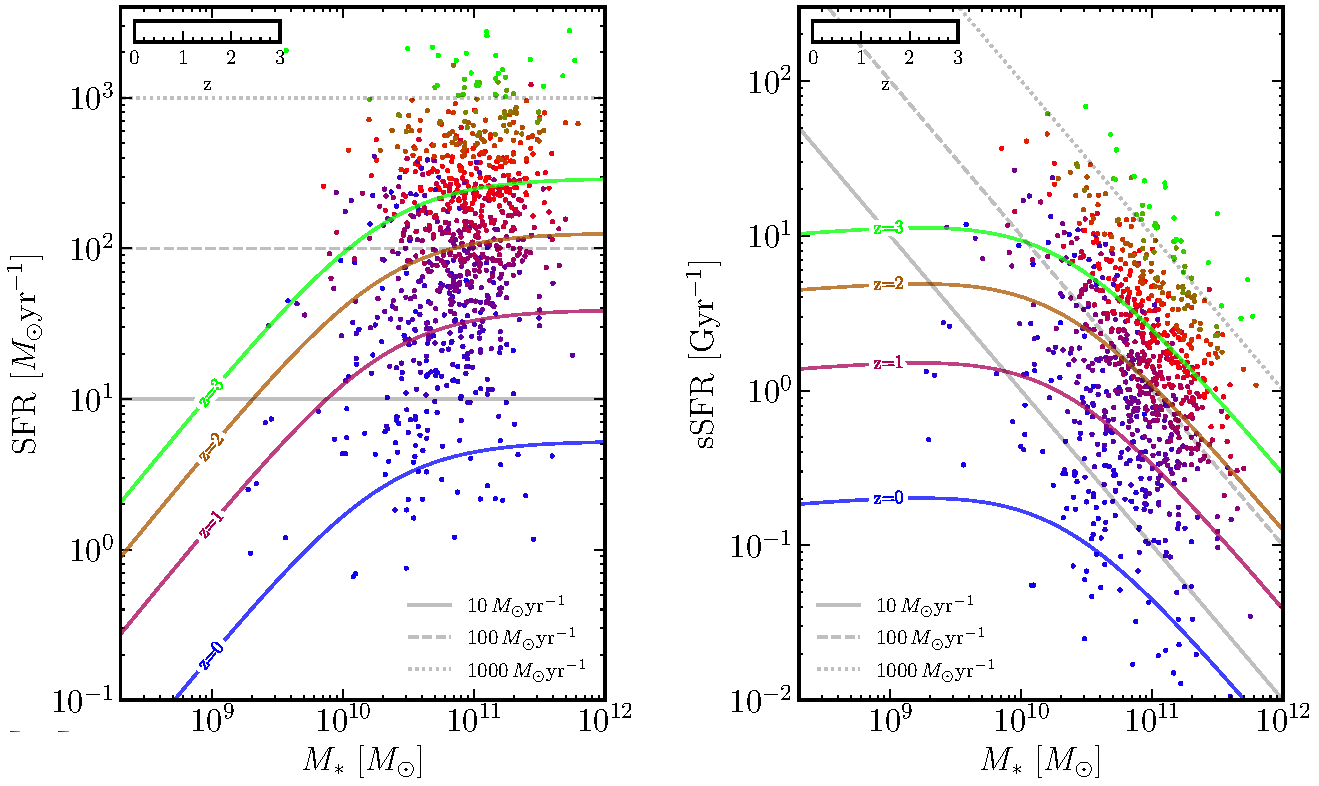
\includegraphics[width=0.9\columnwidth]{Figures/star_formation_ms.pdf}
	\caption{The stellar mass - star formation rate relation (left) and the stellar mass - specific star formation rate (right) at $0 < z < 3$. In both panels the sample of \textit{Herschel}-COSMOS sources is coloured according to their photometric redshift. The solid, dashed and dotted lines mark the loci of constant star formation rates of $10$, $100$ and $1,000\,M_\odot$yr$^{-1}$, respectively. The coloured lines indicate the main sequence for star forming galaxies defined by \citealt{Scoville_2017} at $z = 0, 1, 2$ and $3$. {\color{red}Check why colour in colourbar is removed.}}
	\label{fig:star_formation_ms}
\end{figure}

The left panel of Figure \ref{fig:star_formation_ms} shows that at the redshift of each galaxy, the \textit{Herschel} sources are significantly above the MS in most cases. This result is not necessarily surprising given the SFR limits imposed by large-area \textit{Herschel} surveys. The monotonically increasing limit for IR luminosity with redshift forces a similar trend in the limiting SFR with redshift, causing us to be restricted to observing starbursts or high mass MS galaxies at lower redshifts. For the highest redshifts ($z \gtrsim 2.5$) we measure star formation rates in excess of $1,000\,M_\odot$yr$^{-1}$. The majority of these sources have IR luminosities $> 10^{12.9}\,L_\odot$, which puts them in the same category as the most massive Ultraluminous Infrared Galaxies (ULIRGs, $> 10^{12}\,L_\odot$) and Hyperluminous Infrared Galaxies (HyLIRGs, $> 10^{13}\,L_\odot$) {\color{red}Repeated definitions}. 

We find it constructive to express this figure in terms of the specific star formation rate, sSFR, which provides a fairer comparison among galaxies of different sizes (righthand panel of Figure \ref{fig:star_formation_ms}). The sSFR of our sample informs us about how efficiently the galaxies are forming their stellar mass, relative to their existing stellar content. The sSFR of a galaxy is a useful indicator of the current star formation compared to past star formation since, at a constant rate of <SFR>, the stellar mass is proportional to <SFR> $\times t_{\textrm{age}}$ where $t_{\textrm{age}}$ is the age of the galaxy, ignoring the effects of recycling. This means that if we assume a constant star formation rate, the sSFR of a galaxy scales as the inverse of the age of the galaxy.

The right hand panel shows that the higher mass galaxies have typically lower specific SFRs than less massive ones. There is previous evidence to suggest that the major contribution to star formation in a galaxy starts later for less massive galaxies, which would manifest itself as a higher sSFR. This implies that massive galaxies formed their stars earlier whereas less massive galaxies are still actively star forming, hence their elevated sSFR (e.g. \citealt{Brinchmann_2000}; \citealt{Juneau_2005}; \citealt{Bell_2005}; \citealt{caputi_2006}; \citealt{Reddy_2006}; \citealt{Noeske_2007}). At first sight our sample would be in agreement with this "cosmic downsizing", however, we add the caveat that our $L_{\textrm{IR}}$ limits at each redshift create an sSFR limit diagonal in the sSFR-$M_*$ plane from low mass, high sSFR to high mass, low sSFR. At the lowest redshifts ($z \lesssim 0.5$), the far-infrared survey limits allow us to observe more of the low mass, low sSFR galaxies, including some that sit on the MS. For this subset of galaxies where we have a more complete picture, the correlation between the $\textrm{log}(M_*)$ and specific SFR is $\rho_{\textrm{Spearman}} = -0.28$.

There are no formal, physical definitions for a starburst galaxy, the term is applied to a diverse range of galaxy populations. However, common to all starbursting populations is that they have SFRs that are much higher than their long-term average. We consider a star-forming galaxy to be defined as in a "starbursting phase", if the length of time it would take to form its observed stellar mass is a small fraction of the age of the Universe at the redshift of the galaxy. In this sense, observing these galaxies during an intense period of star formation means we are directly observing these galaxies as they form the bulk of their stellar mass. The total mass of stars in a galaxy would be produced in a timescale given by $\tau = 1/$sSFR, which we standardize by the age of the Universe at the redshift of the galaxy, $t_z$. Figure \ref{fig:tau_against_age} shows that the average doubling timescale is approximately $10\%$ of the age of the Universe, which would imply short starburst duty cycles (dependent on the mass of molecular gas available). It also illustrates that the fraction of time spent in this phase of evolution is likely shorter for higher redshift galaxies - which is to say that at redshifts near the epoch of peak star formation, such galaxies are forming the bulk of their stellar mass more quickly.

\begin{figure}
	\centering
	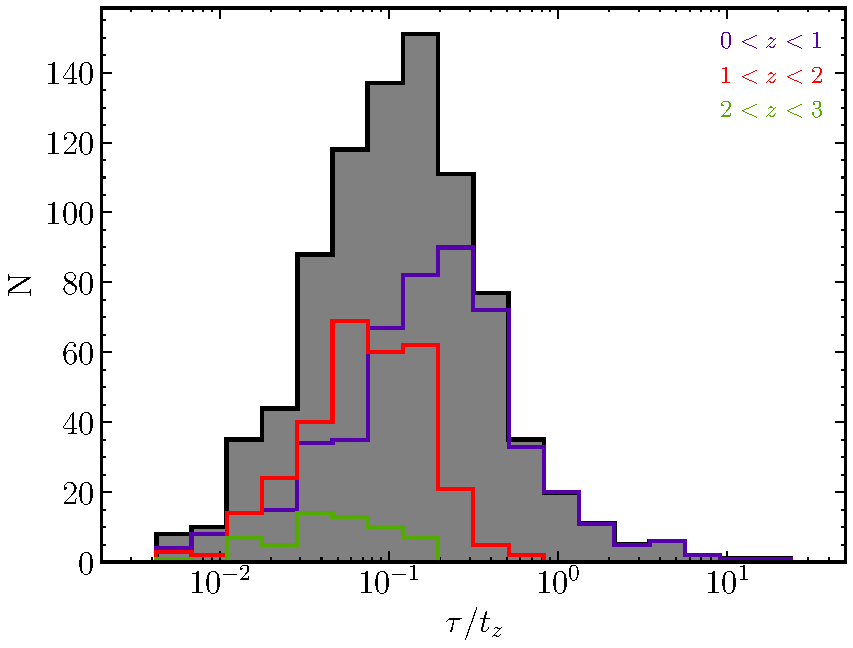
\includegraphics[width=0.75\columnwidth]{Figures/tau_against_age.pdf}
	\caption{The distribution of the doubling timescale, $\tau = 1/$sSFR, divided by the age of the Universe at the redshift of the galaxy. The figure shows that the typical time it would take to form the stellar masses of our \textit{Herschel} galaxies is approximately $10\%$ of the age of the Universe. The purple, red and green lines represent the subsamples at redshift intervals of $0 < z < 1$, $1 < z < 2$ and $2 < z < 3$.}
	\label{fig:tau_against_age}
\end{figure}

The SMGs observed at $z\gtrsim2$ have exceptional star formation rates that make them ideal candidates for being the progenitors to the massive elliptical galaxies in the local Universe. In this scenario, these galaxies represent a fixed stage in the evolutionary sequence toward a local massive, dead elliptical. In this paradigm, two gas-rich disk galaxies collide and ignite an intense starbursting phase due to rapid compression and cooling of the gas. This phase of high SFR produces the vast quantities of dust and the young, radiating blue stars that make this evolutionary stage bright in the far-infrared and sub-mm wavelengths. With limited gas supply and high SFRs, this burst is short-lived ($\sim 10^7 - 10^8\,$yr; {\color{red}REFERENCES}). Star formation ceases, potentially due to the formation of an AGN, and the galaxy secularly evolves to an elliptical galaxy with an old stellar population. Much of this evolutionary connection is based on similarities in the two populations, notably the distribution of their sizes, stellar masses and internal velocities (\citealt{Toft_2014}). {\color{red}Any back-of-envelope calculation that can back this up? Comparison of stellar masses? Today most galaxies with stellar masses $>10^{10.5}\,M_\odot$ are ETGs.} It therefore seems likely that our sample of \textit{Herschel}-detected galaxies are early Universe versions of elliptical galaxies being observed during a rapid mass building phase.

\section{Identifying Multiwavelength Counterparts of SMGs from Blank Fields}

The identification of radio counterparts to \textit{Herschel} sources in COSMOS has shown the efficiency with which we can unambiguously locate at least one very likely optical/infrared association. However, as mentioned earlier, this method is not practical on the scale of the \textit{Herschel} surveys conducted to date and hundreds of thousands of sub-mm sources do not have the depth of radio coverage as in COSMOS or have optical identifications that are not considered significant enough to be called a reliable match. With our high identification rate ($\sim 80\,\%$) we aim to show proof-of-concept for a future program that would be able to identify the characteristics of SMGs in a wide area blank field covered by \textit{Herschel}, using the multiwavelength properties of our sample. Referencing the LR method in Chapter \ref{chapter:Data_Release_3}, we note that this Bayesian analysis of identifying counterparts is dependent on two properties: the radial separation from the sub-mm source and the flux density in a single optical/infrared band (similarly, the frequentist method here is based on two observables: the separation and the radio flux density). While some studies have looked at describing the probability distribution of true counterparts (recall q(m) in Equation \ref{eq:true_counterparts_distribution}) in more than one dimension (e.g. {\color{red}REFERENCE}), this increases the complexity of the problem to one where we define the probability of association between source and counterpart as some surface over an $N$-dimensional surface. We propose that a more efficient method would be to train some machine learning algorithm to detect the signatures of an SMG from the set of observables we typically have in a wide field optical/infrared survey, thus reducing the problem to a binary classification problem. Importantly, such a method can also weight the observables accordingly with their influence on the classification, and thus reducing the chance of overfitting as we might expect from current methods applied to a high-$N$ problem.

The first hurdle is that an effective machine learning algorithm requires a training set that represents a complete census of the target population. Any subpopulation of the target population that is not represented in the training set will not have any chance of being selected by the algorithm. We already know that we are missing $\sim20\,\%$ of the \textit{Herschel} population in the COSMOS field, which, if they had distinctly different properties from the rest of the sample, would not be recovered when applied to future fields. In this case, we have not found evidence to suggest that these objects represent a distinct group of galaxies, and the most obvious explanation for missing IDs, their redshift, does not appear to be the cause. For this reason, we continue to explore the differentiating power of our multiwavelength properties for the 1,053 \textit{Herschel} sources for which we have robust radio IDs, on the assumption that they represent a reasonable description of the full \textit{Herschel}-detected population from $z = 0$ to $z = 3$.

\begin{table}
    \centering
    \begin{tabular}{p{4cm}|p{1.5cm}|p{2cm}|p{2cm}|p{1.5cm}|p{1.5cm}}
        \hline
		\hline
		Instrument / Telescope & Band & Wavelength [$\mu$m] & Band Width [$\mu$m] & $N_{\textrm{SMG}}$ & Percent \\
		\hline
		\hline
		GALEX & FUV & 0.1526 & 0.0224 & 283 & 26.90 \\
		& NUV & 0.2307 & 0.0791 & 475 & 45.15 \\
		\hline
		MegaCam / CFHT & $u$ & 0.3709 & 0.0518 & 847 & 80.51 \\
		\hline
		Suprime-Cam / & $IB427$ & 0.4266 & 0.0207 & 805 & 76.52 \\
		Subaru & $B$ & 0.4488 & 0.0892 & 909 & 86.41 \\
		& $IB464$ & 0.4635 & 0.0218 & 792 & 75.29 \\
		& $g^+$ & 0.4804 & 0.1265 & 874 & 83.08 \\
		& $IA484$ & 0.4851 & 0.0229 & 844 & 80.23 \\
		& $IB505$ & 0.5064 & 0.0231 & 837 & 79.56 \\
		& $IA527$ & 0.5261 & 0.0243 & 835 & 79.37 \\
		& $V$ & 0.5487 & 0.0954 & 904 & 85.93 \\
		& $IB574$ & 0.5766 & 0.0273 & 837 & 79.56 \\
		& $IA624$ & 0.6232 & 0.0300 & 861 & 81.84 \\
		& $r^+$ & 0.6305 & 0.1376 & 915 & 86.98 \\
		& $IA679$ & 0.6780 & 0.0336 & 849 & 80.70 \\
		& $IB709$ & 0.7073 & 0.0316 & 852 & 80.99 \\
		& $NB711$ & 0.7121 & 0.0072 & 845 & 80.32 \\
		& $IA738$ & 0.7361 & 0.0324 & 857 & 81.46 \\
		& $i^+$ & 0.7693 & 0.1497 & 876 & 83.27 \\
		& $IA767$ & 0.7694 & 0.0243 & 848 & 80.61 \\
		& $NB816$ & 0.8150 & 0.0120 & 903 & 85.84 \\
		& $IB827$ & 0.8243 & 0.0343 & 855 & 81.27 \\
		& $z^+$ & 0.8978 & 0.0365 & 913 & 86.79 \\
		& $z^{++}$ & 0.9063 & 0.1335 & 883 & 83.94 \\
        \hline
		Hyper Suprime-Cam / & $g$ & 0.4847 & 0.1383 & 919 & 87.36 \\
		Subaru & $r$ & 0.6219 & 0.1547 & 920 & 87.45 \\
		& $i$ & 0.7699 & 0.1471 & 922 & 87.64 \\
		& $z$ & 0.8894 & 0.0766 & 922 & 87.64 \\
		& $y$ & 0.9761 & 0.0786 & 922 & 87.64 \\
		\hline
		ACS / HST & F814W & 0.8333 & 0.2511 & 613 & 58.27 \\
		\hline
		VIRCAM / & $Y$ & 1.0216 & 0.0923 & 738 & 70.15 \\
		VISTA & $NB118$ & 1.1909 & 0.0112 & 442 & 42.02 \\
		& $J$ & 1.2525 & 0.1718 & 735 & 69.87 \\
		& $H$ & 1.6466 & 0.2905 & 740 & 70.34 \\
		& $K_s$ & 2.1557 & 0.3074 & 740 & 70.34 \\
		\hline
		IRAC / & ch1 & 3.5686 & 0.7443 & 884 & 84.03 \\
		Spitzer & ch2 & 4.5067 & 1.0119 & 883 & 83.94 \\
		& ch3 & 5.7788 & 1.4082 & 881 & 83.75 \\
		& ch4 & 7.9958 & 2.8796 & 876 & 83.27 \\
		\hline
		\hline
    \end{tabular}
    \caption{The UV to IR data in the COSMOS2020 catalogue. The final two columns show he number of \textit{Herschel} sources with an observation in the given photometric band and the fraction of these sources as a percentage.}
    \label{tab:smg_coverage}
\end{table}

Table \ref{tab:smg_coverage} shows the UV-IR coverage provided by COSMOS2020, including the fraction of our SMGs that have observations. In most cases the fraction of our SMGs with an observation at a given band is between $70\%$ and $85\%$. At this time, we have no reason to suspect that the sources that have missing UV-IR photometry are any different to the rest of the population (it is often the case that a source missing observations will not have coverage across the full short wavelength spectrum). In Figure \ref{fig:smg_colours} we plot a range of colour-colour plots that, from top to bottom, progressively samples the UV to IR bands. Given the wide redshift range of our SMGs it is unlikely that we would find any single feature that would help distinguish most of our SMGs from the background galaxies (grey histograms). However, Figure \ref{fig:smg_colours} does show the possible separation between SMGs and non-SMGs that can be made at a given redshift, with the SMGs almost always having redder colours. This is not particularly surprising given the dust reddening that we would expect from these galaxies; previous studies have already illustrated that SMGs are in general red in optical to near-IR colours (e.g. \citealt{Smail_2002}; \citealt{Dannerbauer_2004}; \citealt{Wang_2012}; \citealt{Chen_2016}), resulting in optical colour cuts previously being used to identify possible counterparts (e.g. \citealt{Michalowski_2012b}). The problem with single colour cuts is that the contamination rate from field galaxies is likely to be large.

\begin{figure}
	\centering
	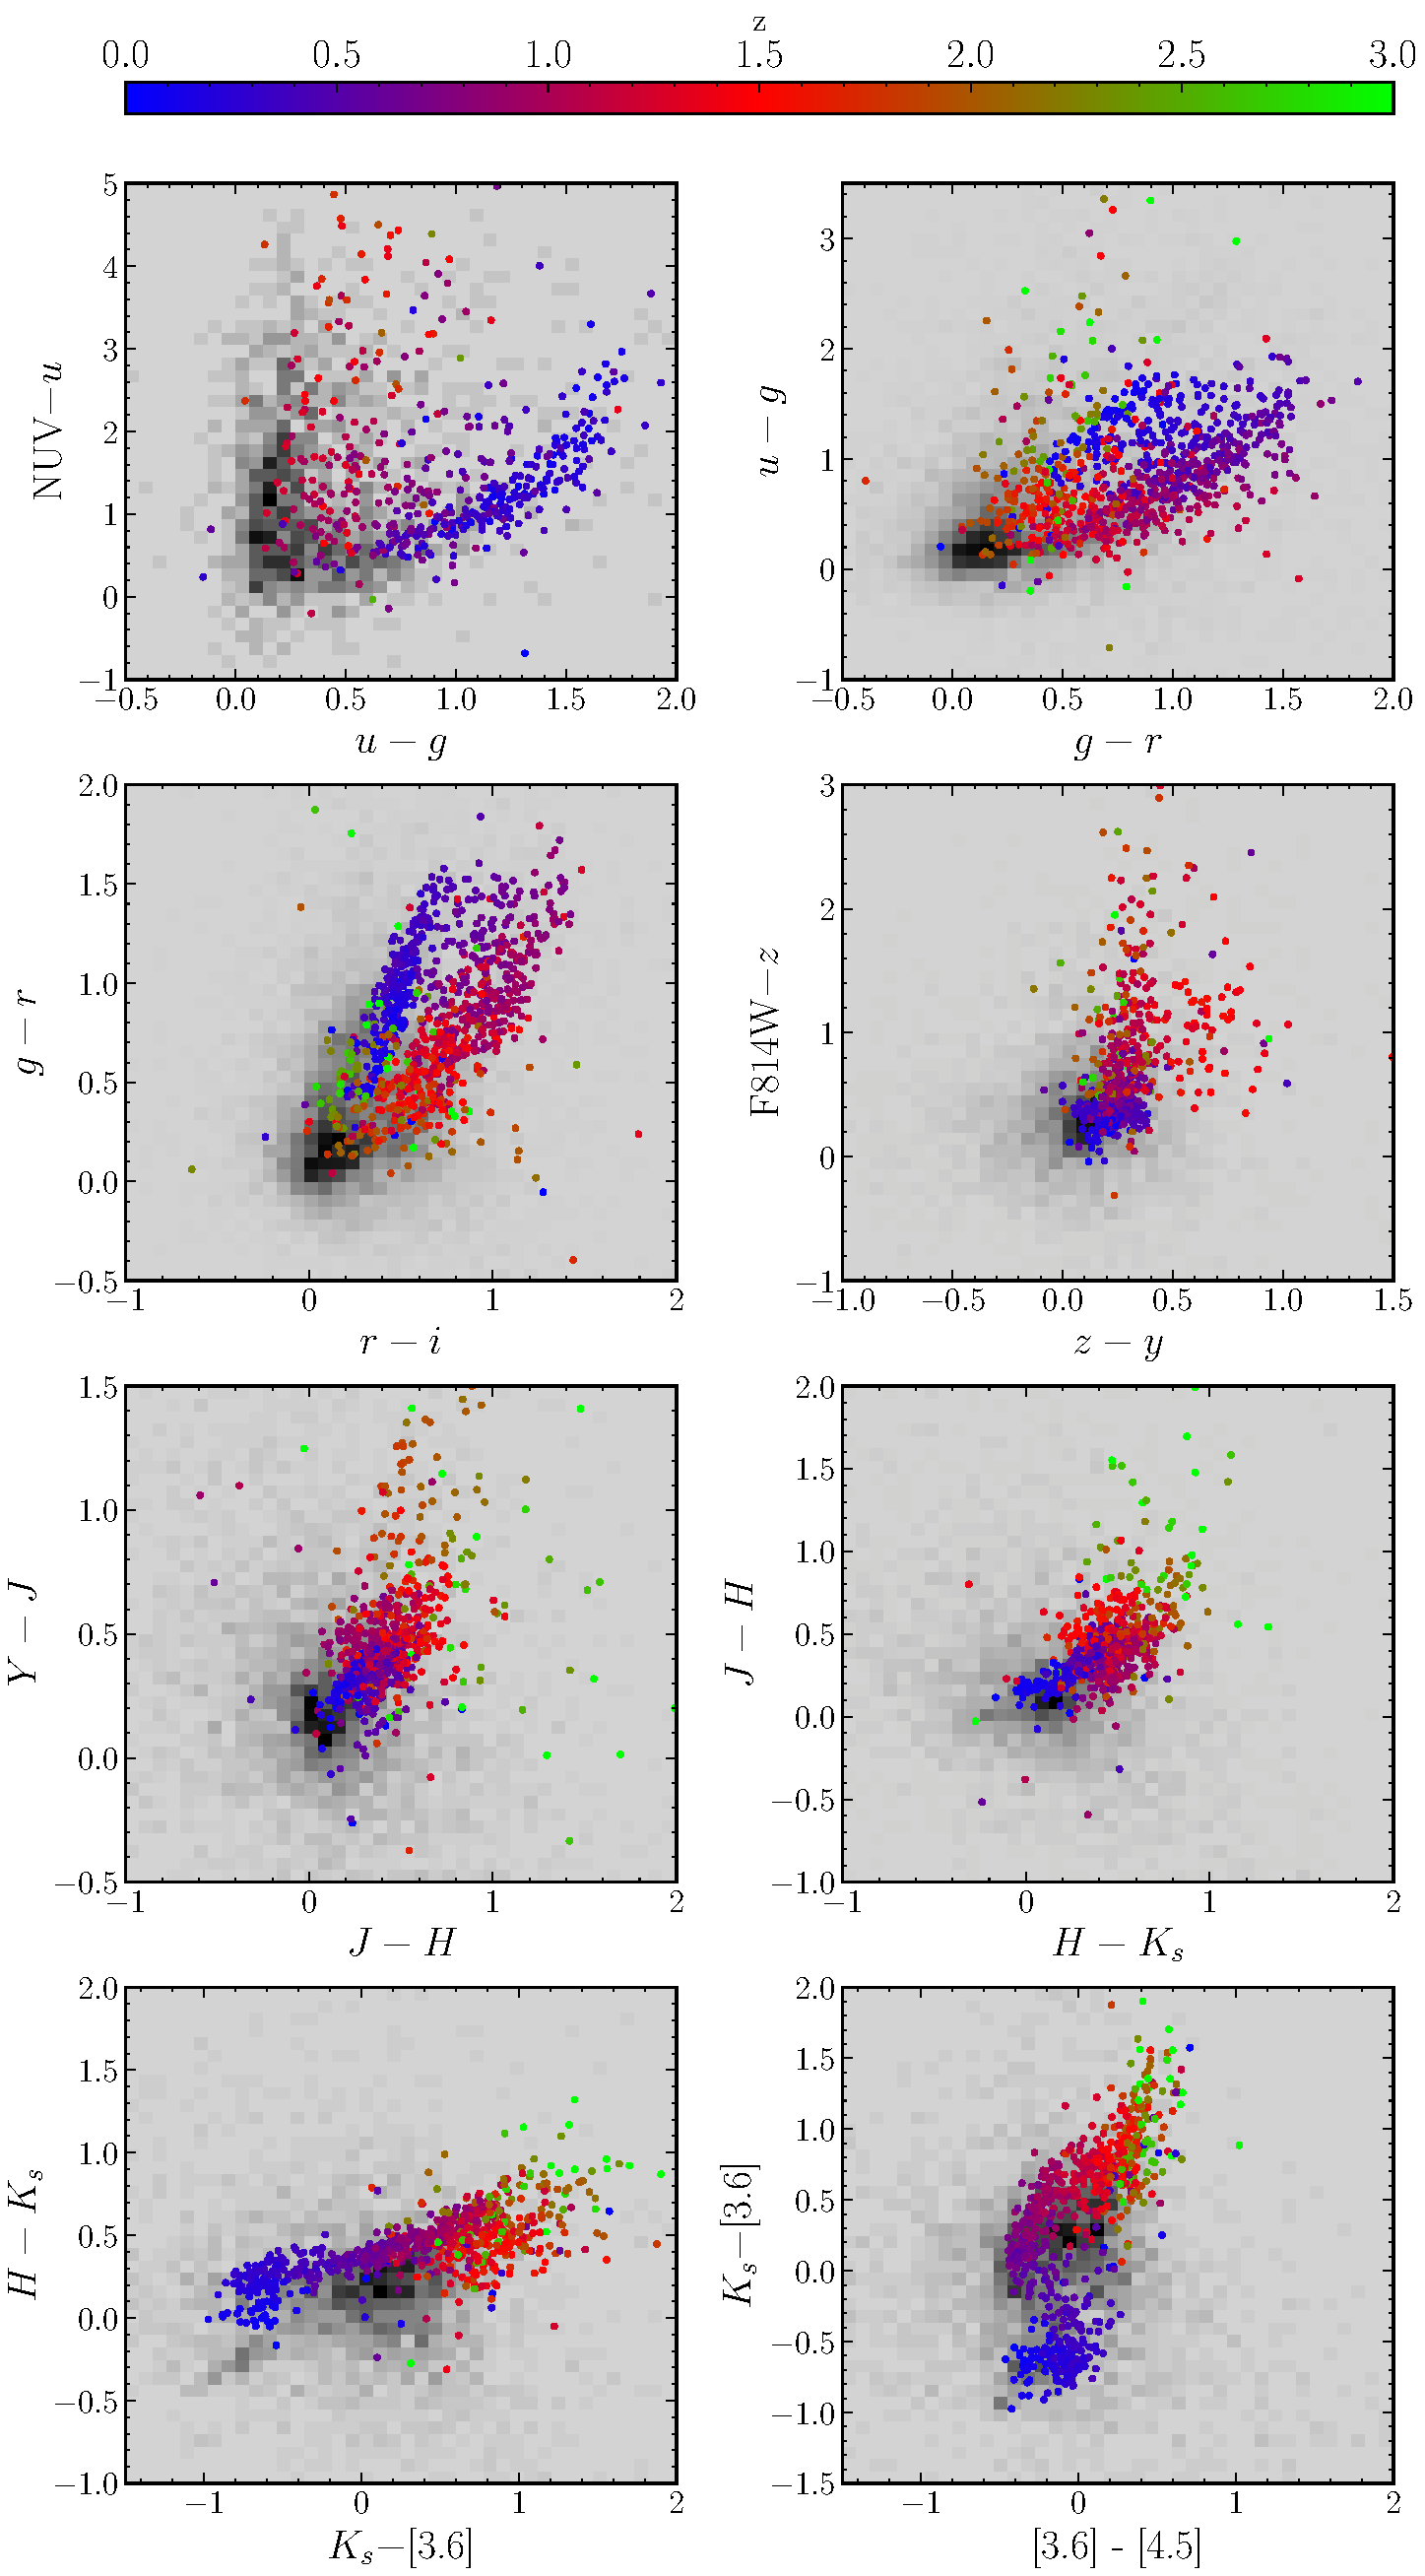
\includegraphics[width=0.85\columnwidth, height=0.9\textheight]{Figures/smg_colours.pdf}
	\caption{A selection of colour-colour spaces for the multiwavelength counterparts to our \textit{Herschel} sources, coloured by their photometric redshift. The 2D histograms (black) show the distribution of the full COSMOS2020 catalogue. The colour-colour plots are selected to traverse the UV to IR spectrum, from the top row to the bottom.}
	\label{fig:smg_colours}
\end{figure}

\textbf{*** This point onwards feels very weak, perhaps unnecessary ***}

We recall in Chapter \ref{chapter:Data_Release_3} that we were able to reliably match $\sim 60\%$ of \textit{Herschel} sources in the South Galactic Pole field of H-ATLAS with a near-infrared counterpart, providing that there was at least one near-IR object on the VIKING image. We propose that had we a priori knowledge about a selection of optical/IR colours of SMGs in comparison to non-SMGs, we might be able to use this information to improve on our recovery percentage in the cases where we are still unsure whether a possible counterpart is the true ID or not. Assuming we could produce some useful Machine Learning algorithm that could locate SMGs from a blank field, we would ideally like to directly compare our results with the current standard method, like the Likelihood Ratio technique. However, the efficacy of such an algorithm will be heavily dependent on the surface density of SMGs to non-SMGs and their redshift distributions. In order to make a fair comparison between two identification techniques, we would have to faithfully recreate a mock version of the optical/IR catalogue. Instead, to illustrate how useful additional photometric coverage would be in identifying dusty galaxies, we start from the assumption that we have already detected a \textit{Herschel} source and observed nearby optical/IR counterparts. In our simple situation our question is - if there is one counterpart near the sub-mm source, how confident can we be in our binary classification of SMG or non-SMG?

In Figure \ref{fig:smg_nonsmg} we show the histograms of different observed properties (the spatial offset between the sub-mm source position and the optical galaxies and a selection of colours). As would be expected, the most definitive way of deciphering between SMGs and non-SMGs is in the separation between source and counterpart. To illustrate how well each observable could be used individually, we show the SMG fraction in the bottom panel, defined as $f_\textrm{SMG} = N_\textrm{SMG}/(N_\textrm{SMG}+N_\textrm{non-SMG})$. We estimate this fraction by randomly selecting $100$ of our SMGs and $100$ other galaxies from the COSMOS2020 catalogue. We measured $f_\textrm{SMG}$ for $1,000$ iterations and plotted the median values as a function of the observed quantity. In regions where SMGs dominate non-SMGs the fraction would tend to one. If the two populations occupy distinctly different ranges, then there would be a sharp change in $f_\textrm{SMG}$. We model $f_\textrm{SMG}$ with a sigmoid function of the form $\alpha/(1+e^{\beta(x-\gamma)})$ where $x$ is the observable quantity and $\alpha$, $\beta$ and $\gamma$ are constants. As we might predict, the most compelling observable quantity for distinguishing the two populations is the spatial offset; at low radii the fraction is essentially one. The figure also demonstrates that select colours are particularly effective at distinguishing SMGs from non-SMG galaxies. It is clear that the overlap between SMGs and non-SMGs for any property can be substantial, but a combination of them would efficiently reduce the contamination from field galaxies.

\begin{figure}
	\centering
	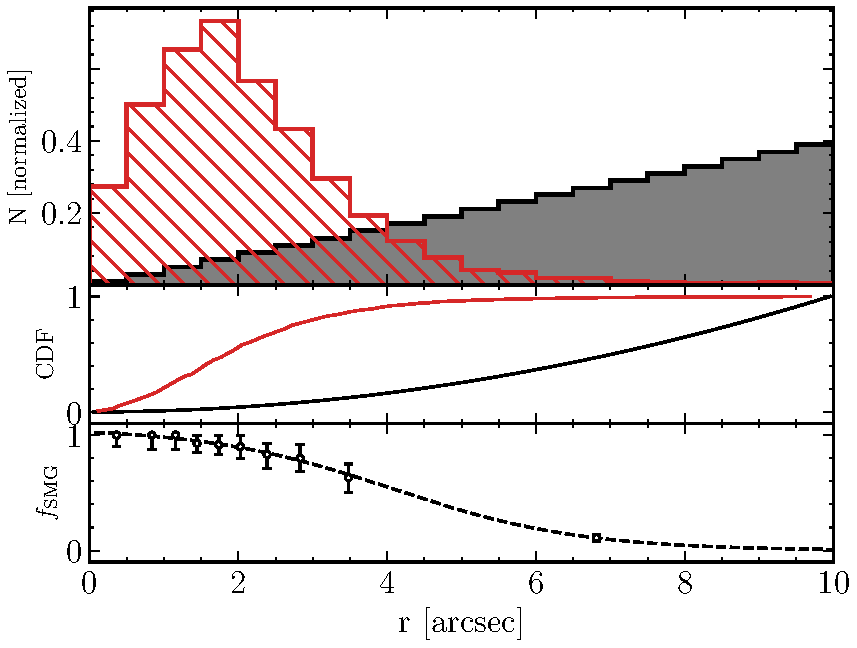
\includegraphics[width=0.49\columnwidth, height=0.3\textheight]{Figures/offset_smg.pdf}
	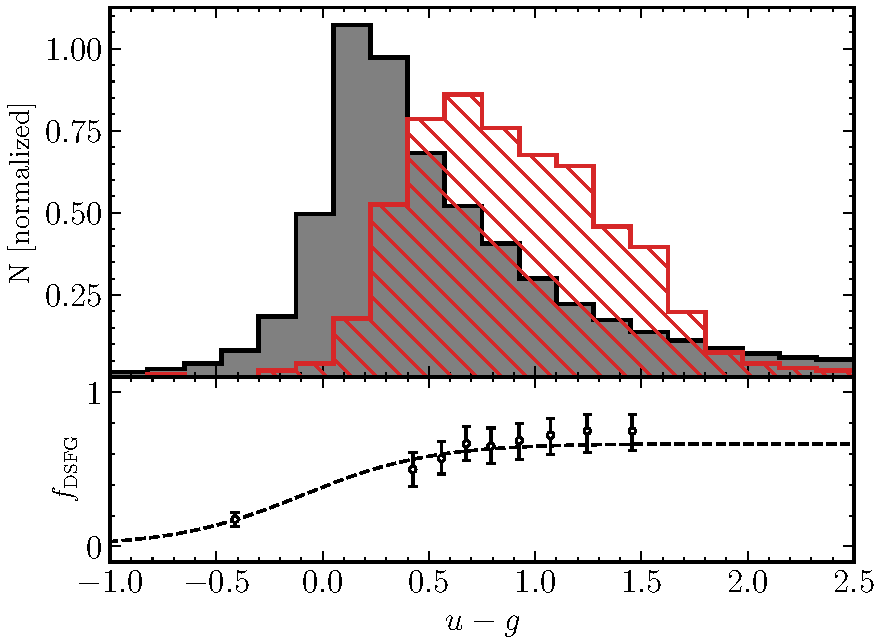
\includegraphics[width=0.49\columnwidth, height=0.3\textheight]{Figures/ug_smg.pdf}
	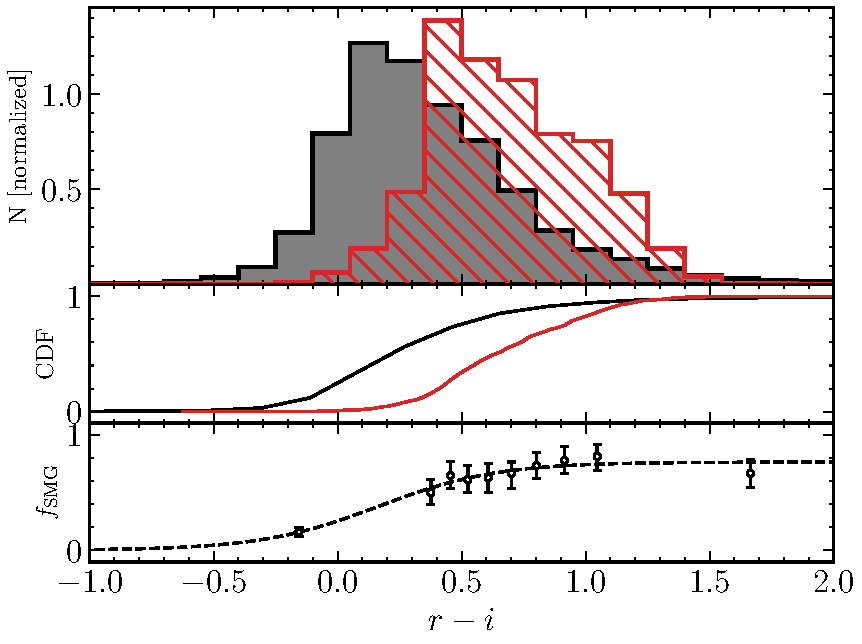
\includegraphics[width=0.49\columnwidth, height=0.3\textheight]{Figures/ri_smg.pdf}
	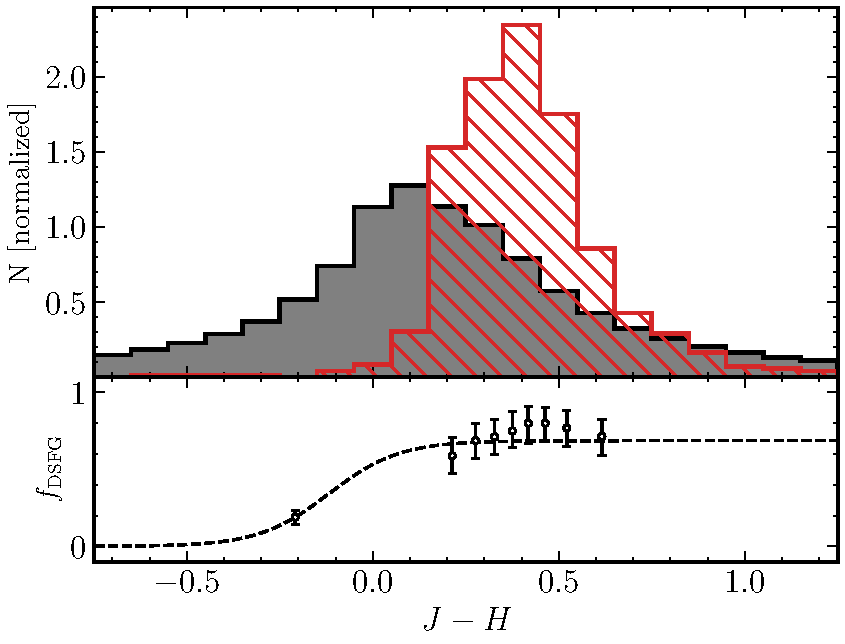
\includegraphics[width=0.49\columnwidth, height=0.3\textheight]{Figures/JH_smg.pdf}
	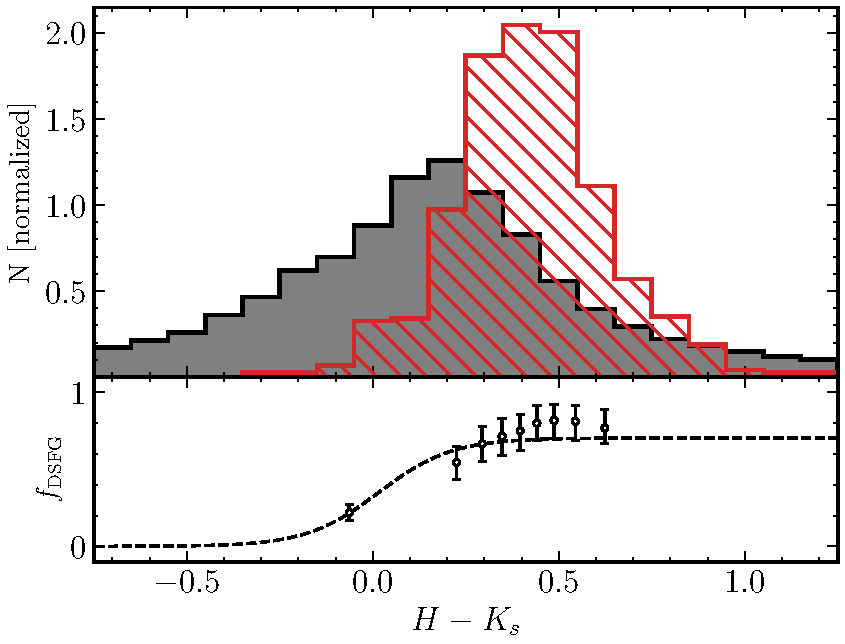
\includegraphics[width=0.49\columnwidth, height=0.3\textheight]{Figures/HK_smg.pdf}
	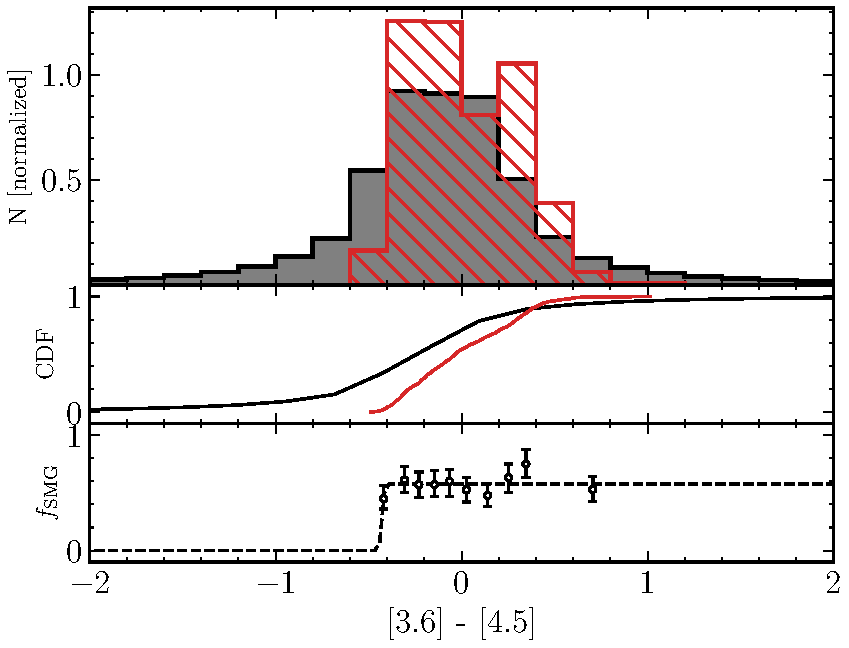
\includegraphics[width=0.49\columnwidth, height=0.3\textheight]{Figures/3645_smg.pdf}
	\caption{{\color{red}Caption}}
	\label{fig:smg_nonsmg}
\end{figure}

\section{Conclusion}